../cictikz/src/cictikz/data/tex/cictikz_preamble.tex

% The same staircase read as a converter: the width of each fully
% traversed code against the ideal 4.75 K step, from the temperature
% chamber sweep. GR06, with no clock anywhere in its path, has no
% equivalent.
%
% Generated by py/tikzplot.py. Edit the script in ex/ that
% produced it and re-run that, not this file.

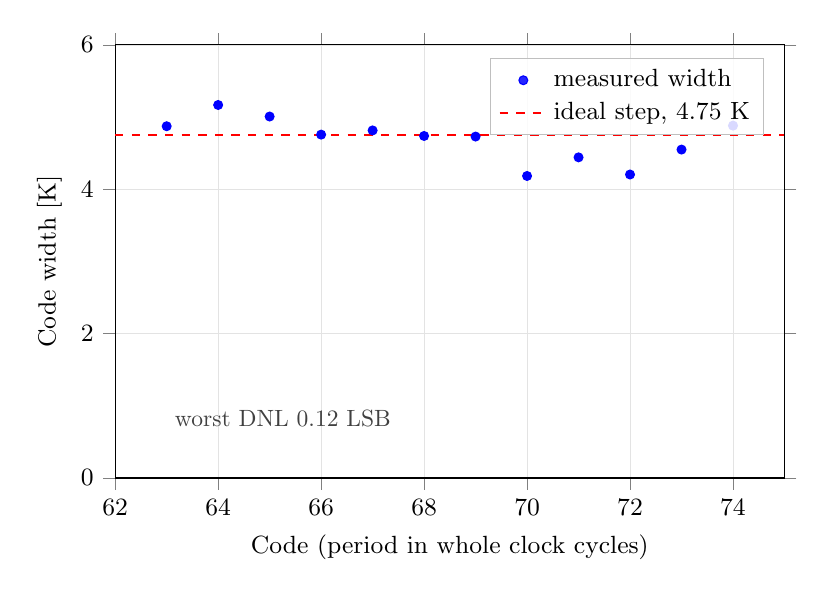
\begin{tikzpicture}[thick]

\begin{axis}[
  width=8.5cm,
  height=5.5cm,
  scale only axis,
  grid=both,
  grid style={gray!22, very thin},
  tick align=outside,
  tick label style={font=\small},
  label style={font=\small},
  title style={font=\small, yshift=-1mm},
  legend cell align=left,
  legend style={font=\small, draw=gray!50, fill=white, fill opacity=0.85, text opacity=1},
  xlabel={Code (period in whole clock cycles)},
  ylabel={Code width [K]},
  xmin=62,
  xmax=75,
  ymin=0,
  ymax=6,
  legend pos=north east
]
\addplot[blue, only marks, mark=*, mark size=1.6pt, mark=none] coordinates {(63,4.8734) (64,5.1678) (65,5.0079) (66,4.7571) (67,4.8154) (68,4.7385) (69,4.7302) (70,4.1841) (71,4.442) (72,4.2045) (73,4.5501) (74,4.8816)};
\addlegendentry{measured width}
\addlegendimage{red, thick, dashed}
\addlegendentry{ideal step, 4.75 K}
\draw[red, thick, dashed] ({rel axis cs:0,0} |- {axis cs:0,4.7478}) -- ({rel axis cs:1,0} |- {axis cs:0,4.7478});
\node[anchor=south west, gray!50!black, scale=0.85, align=left] at (axis cs:63,0.6) {worst DNL 0.12 LSB};
\end{axis}

\end{tikzpicture}
\end{document}
